\subsubsection{Server structure}
When setting up the server side, the project got divided into different blocks. Each block would have it's own use case as far as possible. If done correctly there is many benefits by splitting code into different blocks. The standard way of splitting code is to follow SOLID (S: Single responsibility principle, O: Open–closed principle, L: Liskov substitution principle, I: Interface segregation principle, D: Dependency inversion principle). If this is followed correctly it will give the advantages of MURDER(M: Maintainability, U: Understandability, R: Reuseability, D: Debugability, E: Extensibility, R: Regression). Examples of this can be seen in how the socket functions are split up into categories with for example client function, admin functions, feide functions split into their own file and then imported where they are needed. The same can be seen in the database functions, where get, insert, update and delete functions are split into their own files to make development easier. When it comes to extensibility, the server is written to be able to scale up with more question types in a very easy manner. The way the server handles generating a solution, validating a question og checking an answer is written into their own files based on question type. This makes it so that if another question type should be added, the developer should only need to add a couple of lines in each master file to make it work. It is also required for the developer to implement their algorithms in their sepperate files.
\begin{figure}[h]
    \centering
    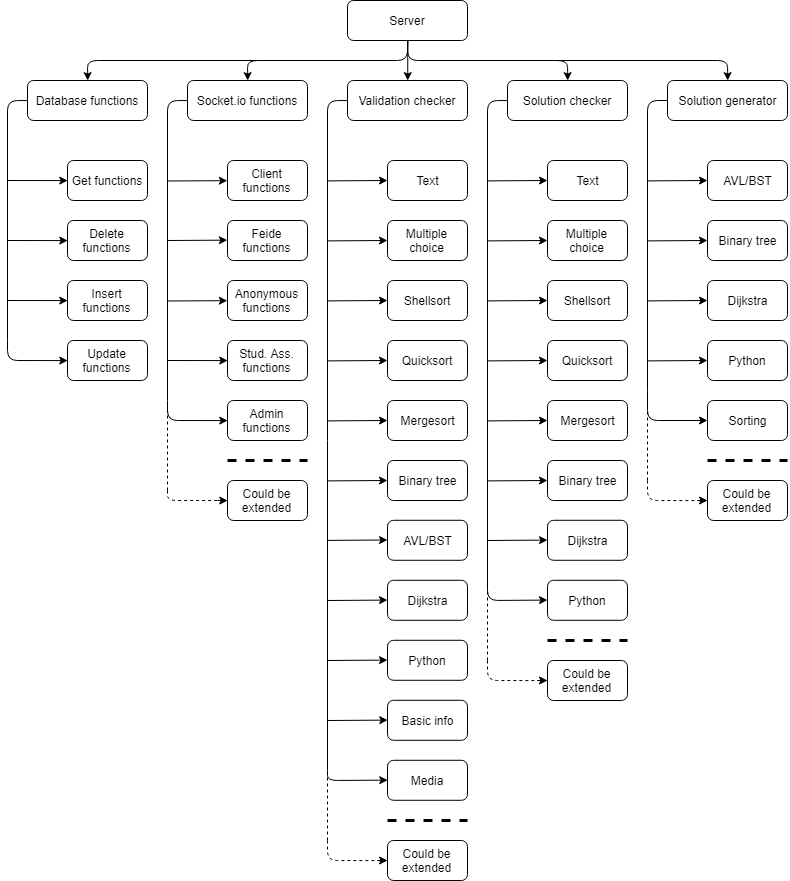
\includegraphics[width=\linewidth]{diagrammer/serverStructure}
    \caption{This is a diagram displaying the server structure and how the code is divided up into different sub files}
    \label{fig:serverStructure}
\end{figure}